\thispagestyle{cackithitoannone}
\pagestyle{cackithitoan}
\everymath{\color{cackithi}}
\graphicspath{{../cackithi/pic/}}
\begingroup
\AddToShipoutPicture*{\put(0,616){
\includegraphics[width=19.3cm]{../bannercackithi}}}
\AddToShipoutPicture*{\put(100,555){
\includegraphics[scale=1]{../tieude.pdf}}}
\centering
\endgroup
\vspace*{155pt}

\begin{multicols}{2}
	Kỳ thi Olympic Toán học Mát--xcơ--va đầu tiên được tổ chức vào năm $1935$, theo sáng kiến của Hiệp hội Toán học Mátxcơva bởi Bộ Giáo dục, Đại học Quốc gia Mát--xcơ--va và Sở Giáo dục Thành phố. Ban tổ chức Olympic này bao gồm những người như Pavel Aleksandrov, Sergei Sobolev, Lev Shnirelman, Andrey Kolmogorov, những nhà toán học lỗi lạc thời bấy giờ. Kể từ năm $1967$, Olympic Toán học Mát--xcơ--va đã trở thành một cấp trong Olympic Toán toàn Nga (và sau này là toàn Liên bang).
	\begin{figure}[H]
		\vspace*{-5pt}
		\centering
		\captionsetup{labelformat= empty, justification=centering}
		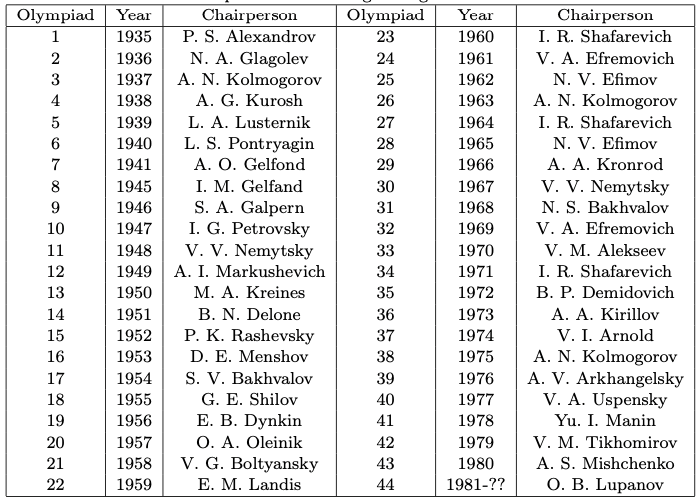
\includegraphics[width= 1\linewidth]{1}
		\caption{\small\textit{\color{cackithi}Các trưởng ban tổ chức MMO từ $1935$ đến $1981$.}}
		\vspace*{-10pt}
	\end{figure}
	Năm $1980$, Hội Toán học Mát--xcơ--va bị loại ra khỏi ban tổ chức Olympic Toán học Mát--xcơ--va và Toàn Nga. Nikolai Konstantinov, một trong những người lãnh đạo phong trào Olympic, đã khởi xướng ra Kỳ thi giữa các thành phố (Tournament of the town) vào năm $1981$, một kỳ thi Olympic về cơ bản giống với Olympic toán học Moscow, nhưng được tổ chức cho học sinh từ các thành phố khác nhau đến từ các quốc gia khác nhau.  
	\vskip 0.1cm
	Trong thời kỳ Xô Viết, kỳ thi đã có những ảnh hưởng to lớn tới sự phát triển của nền toán học Xô Viết. Các nhà toán học lớn nhất của Liên Xô ở Mát--xcơ--va đều đã từng tham gia tổ chức kỳ thi với tư cách trưởng ban tổ chức. 
	\vskip 0.1cm
	Năm $1993$, quyền tổ chức Olympic Toán Mát--xcơ--va được trả lại cho Hội Toán học Mát--xcơ--va. Năm $1994$, Festival Toán bắt đầu được tổ chức -- một phiên bản của kỳ thi dành cho học sinh lớp $6-7$.
	\vskip 0.1cm
	Năm $2008$, sau quy định mới về Olympic toàn Nga, Olympic Mát--xcơ--va đã mất tư cách là một kỳ thi của Olympic toàn Nga và trở thành một Olympic độc lập.
	\vskip 0.1cm
	Ngày nay, Olympic Toán Mát--xcơ--va là một kỳ thi Olympic mở, hơn $4{.}000$ học sinh lớp $8-11$ từ Mát--xcơ--va, St. Petersburg, Dolgoprudny, Kirov, Kharkov, Chernogolovka và các thành phố khác của không gian hậu Xô Viết tham gia.
	\vskip 0.1cm
	Các bài toán tại MMO đã được tập hợp trong cuốn sách ``Olympic Toán Mát--xcơ--va" xuất bản năm $1986$ bởi các tác giả G. A. Galperin và A. C. Tolpygo. Cuốn sách này được dịch sang tiếng Anh đồng thời bổ sung nhiều đề thi và lời giải năm $1997$. 
	\begin{figure}[H]
		\vspace*{5pt}
		\centering
		\captionsetup{labelformat= empty, justification=centering}
		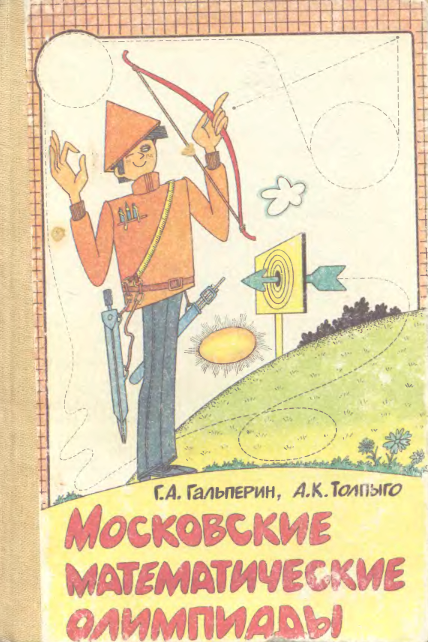
\includegraphics[width= 1\linewidth]{2}
		\caption{\small\textit{\color{cackithi}Bìa cuốn sách ``Olympic Toán Mát--xcơ--va, $1986$.}}
		\vspace*{-10pt}
	\end{figure}
	Để bạn đọc có thể hiểu được phần nào mục đích, ý nghĩa, nguyên tắc cũng như phương thức tổ chức kỳ thi, cách chuẩn bị cho kỳ thi, chúng tôi xin trích giới thiệu Lời tựa của hai tác giả G. A. Galperin và A. C. Tolpygo trong cuốn sách nói trên\footnote[1]{\color{cackithi}Một số tiêu đề bên dưới do tác giả bài viết này đặt.}.
	\vskip 0.1cm
	\textbf{\color{cackithi}Olympic toán có cần không?}
	\vskip 0.1cm 
	Nhiều nhà toán học ở Nga không hài lòng với việc thi giải một số bài toán trong năm giờ đồng hồ tại một kỳ thi Olympic. Họ phản đối sự kết hợp giữa thể thao và khoa học này: nhiều người chiến thắng sau này đã không đạt được nhiều thành tích trong học tập như họ từng đoạt được trong loại hình ``thể thao toán học" thực sự rất cụ thể này. Ngược lại, nhiều người không bao giờ có thể thành công dưới sức ép của một kỳ sau đó lại chứng tỏ họ là những người tài năng và hiệu quả nhất. Đúng là những vấn đề của toán học thực tế cần nhiều tháng và nhiều năm, chứ không phải mấy giờ, để có một bước tiến.
	\vskip 0.1cm
	Tuy nhiên, đối với nhiều học sinh, ý tưởng về một cuộc thi rất hấp dẫn, và các em có thể tham gia chỉ vì mục đích của nó và từ đó khám phá xem Toán học (không chỉ là môn toán) có thể đa dạng và thú vị như thế nào. Sau đó, người ta có thể tìm thấy rất nhiều hoạt động toán học hiệu quả hơn so với các cuộc thi: đọc sách toán học chỉ là một. Nhưng cần phải có bước đầu tiên, và các kỳ thi Olympic, cũng như các bài toán kiểu Olympic trong các câu lạc bộ toán học ở trường, v.v., sẽ giúp thực hiện điều đó.
	\vskip 0.1cm
	Ở Mát--xcơ--va, nhóm các giáo sư và nghiên cứu sinh từng khởi xướng các kỳ thi Olympic cũng đã thiết lập một truyền thống về ``câu lạc bộ toán học" -- các cuộc gặp gỡ hàng tuần của học sinh tại trường Đại học, nơi họ có thể tham dự một bài giảng, giải quyết một số vấn đề, báo cáo tiến trình của họ và nhận được lời khuyên. Nhiều vấn đề lần đầu tiên được đề xuất tại Olympic sau đó đã trở thành ``văn hóa dân gian của các câu lạc bộ" và được dạy cho nhiều thế hệ.
	\vskip 0.1cm
	Sử dụng những bài toán này theo cách này có lẽ sẽ tốt hơn nhiều, bởi vì học sinh có thể lựa chọn giữa: cạnh tranh với những người khác về số lượng bài toán được giải, hoặc chỉ giải một bài khó duy nhất. Do đó, các loại tâm lý khác nhau có thể được đáp ứng đúng cách mà không làm tổn thương bất kỳ ai. (Thất bại trong cuộc thi Olympic có thể là nguyên nhân gây ra rối loạn tâm lý nghiêm trọng trong toàn bộ cuộc sống tương lai.)
	\vskip 0.1cm
	\textbf{\color{cackithi}Làm gì khi không giải được một bài toán khó?}
	\vskip 0.1cm 
	Bạn phải biết rằng một số bài toán trong kỳ thi Olympic rất khó. Một số bài thậm chí khó tới mức trong $5$ giờ của kỳ thi, không một học sinh nào ở thành phố $10$ triệu dân Moscow tìm ra được lời giải đúng. Một bài toán như vậy có thể làm kinh ngạc ngay cả những người có bằng Tiến sĩ. Vì vậy, bạn không nên coi bản thân là không đủ năng lực nếu bạn không giải được bài toán ngay cả sau một tuần vật lộn.
	\vskip 0.1cm
	Nhưng bạn không nên sợ hãi! Lời khuyên của chúng tôi: hãy đặt một bài toán khó sang một bên trong một thời gian thay vì vội vàng tìm đến lời giải ngay sau lần tấn công đầu tiên không thành công.
	\vskip 0.1cm
	\textbf{\color{cackithi}Thế nào là cách luyện tập hiệu quả nhất?}
	\vskip 0.1cm
	Không giống như bài tập trong sách giáo khoa thông thường, một bài toán thực sự cần phải được nghiền ngẫm: người ta phải tìm ra ít nhất một cách để giải quyết nó. Do đó, hãy bắt đầu với những bài toán dễ hơn. Đừng giải quyết tất cả các bài toán một cách tuần tự; đây không phải là bài tập về nhà, hãy chọn những bài toán bạn thấy thú vị.  Nếu bạn không thể giải quyết bài toán, hãy thử một bàit toán tương tự nhưng dễ dàng hơn và giải quyết nó. Nếu bạn thậm chí không thể làm điều đó, hãy tham khảo lời giải. Nhưng cố gắng đừng ``nuốt chửng" lời giải mà hãy đọc nó một cách chậm rãi, như một câu chuyện trinh thám mà bạn cố đoán diễn biến tiếp theo của suy nghĩ. Cuối cùng, hãy xem xét giải pháp ``tổng thể": ý tưởng thúc đẩy chính của nó là gì và quan trọng nhất là làm cách nào để đạt được nó.
	\vskip 0.1cm
	Để hiểu sâu hơn về một lời lời giải, hãy tự hỏi: ở giai đoạn nào của chứng minh, người ta đã sử dụng các dữ kiện đã cho? Liệu khẳng định có còn đúng nếu chúng ta nới lỏng hoặc bỏ qua một điều kiện? Khẳng định ngược lại có đúng không? Điều quan trọng không phải là số lượng các bài toán được giải quyết mà là sự hiểu biết sâu sắc về lời giải của chúng, những kiến thức mới thu lượm được. 
	\vskip 0.1cm
	Hãy nhớ rằng một câu trả lời, như ``Có", ``Không bao giờ" hoặc ``Năm trăm linh năm", không phải là một lời giải, ngay cả khi chúng đúng. Bạn cần lời giải thích cho tất cả các khẳng định, nói một cách rõ ràng không là: hãy cố gắng giải thích mọi thứ.  
	\vskip 0.1cm
	\textbf{\color{cackithi}Lời khuyên cho các bạn tham gia một kỳ thi Olympic}
	\vskip 0.1cm
	$1.$ Đọc tất cả các bài toán được đưa ra và sắp xếp chúng theo thứ tự bạn sẽ giải. Hãy nhớ rằng thứ tự trong đề đưa ra thường phù hợp với độ khó của chúng theo quan điểm của người soạn đề.
	\vskip 0.1cm
	$2.$ Nếu bài toán có cách giải quá dễ, thì rất có thể bạn đã hiểu sai đề bài hoặc giải sai.  
	\vskip 0.1cm
	$3.$ Nếu bạn không thể giải quyết vấn đề, hãy cố gắng đơn giản hóa nó: tạo các số nhỏ hơn, xem xét các trường hợp cụ thể, v.v. , vân vân, hoặc giải ``ngược", dùng phản chứng, thay thế các số bởi các biến số, hoặc ngược lại, \linebreak v.v..
	\vskip 0.1cm
	$4.$ Nếu không quyết định được liệu một khẳng định có đúng hay không, hãy thử lần lượt chứng minh và phủ định nó.
	\vskip 0.1cm
	$5.$ Đừng mắc vào một bài toán quá lâu: thỉnh thoảng hãy nghỉ ngơi và đánh giá vị trí của bạn. Nếu bạn có tiển triển trong lời giải, hãy tiếp tục, nếu không, hãy bỏ qua bài toán này một lát.
	\vskip 0.1cm
	$6.$ Nếu mệt mỏi, hãy thư giãn ngay lập tức (nhìn lên bầu trời và chiêm ngưỡng sự vô tận hoặc đi dọc hành lang).
	\vskip 0.1cm
	$7.$ Sau khi giải quyết xong bài toán, hãy viết lời giải một cách nghiêm túc theo yêu cầu, không phải như một bức thư gửi cho bạn bè. Điều này sẽ giúp kiểm tra các lập luận và sẽ tao hứng khởi để giải các bài toán khác.
	\vskip 0.1cm
	$8.$ Mỗi ý tưởng nên được ghi lại ngay cả khi nó có vẻ hiển nhiên. Do đó, sẽ thuận tiện khi diễn đạt lời giải dưới dạng một loạt các phát biểu (bổ đề).
	\vskip 0.1cm
	$9.$ Học sinh hiếm khi đọc lại sản phẩm của chính mình để cố gắng đặt mình vào vị trí của ban giám khảo: liệu có ai có thể hiểu bất cứ điều gì bạn viết không?"
	\vskip 0.1cm
	\columnbreak
	\textbf{\color{cackithi}Một số bài toán trong Olympic toán học Mát--xcơ--va lần thứ LXXXIII}
	\vskip 0.1cm 
	\textbf{\color{cackithi}Lớp} $\pmb{6.}$ Trên bảng viết các số $2, 3, 4, ..., 29, 30$. Bạn phải nộp một rup để xóa đi một số bất kỳ cùng với tất cả các ước số của nó. Hỏi số rub nhỏ nhất cần thiết để xóa đi tất cả \linebreak các số.
	\vskip 0.1cm
	\textbf{\color{cackithi}Lớp} $\pmb{7.}$ Hỏi hình dưới đây (có tên gọi là ``lạc đà") có thể được chia
	\vskip 0.1cm
	$a)$ dọc theo các đường lưới;
	\vskip 0.1cm
	$b)$ không nhất thiết phải dọc theo các đường lưới
	\vskip 0.1cm
	thành $3$ phần, để từ đó có thể ghép thành một hình vuông?
	\begin{figure}[H]
		\vspace*{-10pt}
		\centering
		\captionsetup{labelformat= empty, justification=centering}
		\begin{tikzpicture}[cackithi,scale=0.7]
			\draw (0,0) grid (10,8);
			\draw[line width=1.5pt,red] (2,1) -- (2,5) -- (1,5) -- (1,6) -- (2,6) -- (2,7) -- (3,7) -- (3,5) -- (4,5) -- (4,4) -- (5,4) -- (5,5) -- (6,5) -- (6,6) -- (7,6) -- (7,7)-- (8,7) -- (8,6) --(9,6) --(9,1) -- (8,1) --(8,2)--(7,2)--(7,4) --(6,4)--(6,3)--(4,3) --(4,2)--(3,2)--(3,1)--(2,1); 
		\end{tikzpicture}
%		\vspace*{-5pt}
	\end{figure}
	\textbf{\color{cackithi}Lớp} $\pmb{8.}$ Cho một số tự nhiên $N$. Vera thực hiện các thao tác sau với nó: đầu tiên, nó cộng thêm $3$ cho đến khi nhận được số chia hết cho $5$ (nếu ban đầu $N$ chia hết cho $5$ thì không cần cộng thêm). Vera chia kết quả cho $5$. Sau đó, cô ấy thực hiện các thao tác tương tự với số mới nhận được. Những số nào không thể được sử dụng để có được số $1$ từ một quá trình như vậy?
	\vskip 0.1cm
	\textbf{\color{cackithi}Lớp} $\pmb{9.}$ Từ sáu que tính với độ dài đôi một khác nhau có thể xếp được thành hai hình tam giác (ba que trong mỗi hình). Hỏi có thể luôn xếp được từ sáu que tính đó một tam giác mà các cạnh của nó lần lượt bao gồm một, hai và ba que không?
	\vskip 0.1cm
	\textbf{\color{cackithi}Lớp} $\pmb{10.}$ Tồn tại hay không một đa giác nội tiếp $19$ cạnh mà không có hai cạnh cùng độ dài và tất cả các góc được biểu thị bằng những số nguyên độ?
	\vskip 0.1cm
	\textbf{\color{cackithi}Lớp} $\pmb{11.}$ Có $2n$ số nguyên liên tiếp được viết lên bảng. Mỗi bước, bạn có thể chia các số đã viết thành các cặp theo cách tùy ý và thay thế mỗi cặp bằng tổng và hiệu của các số trong cặp này (không cần thiết phải trừ số nhỏ hơn cho số lớn hơn; tất thay thế xảy ra cùng một lúc). Chứng minh rằng sẽ không bao giờ có $2n$ số liên tiếp trên bảng nữa.
\end{multicols}
\newpage
\begingroup
\AddToShipoutPicture*{\put(150,700){
\includegraphics[scale=1]{../tieude1.pdf}}}
\centering
\endgroup
\vspace*{5pt}

\begin{multicols}{2}
	Trong phần đầu chuyên mục, chúng tôi sẽ trình bày với các bạn lời giải của các bài toán trong kỳ thi Olympic Toán học vùng Cáp--ca năm học $2022$ (Caucasus Math Olympiad), đăng trong số báo tháng $12/2022$. 
	\begin{figure}[H]
		\vspace*{-5pt}
		\centering
		\captionsetup{labelformat= empty, justification=centering}
		
\includegraphics[width= 1\linewidth]{gocolympic}
		\vspace*{-10pt}
	\end{figure}
	{\bf\color{cackithi} OC$\pmb{28.}$} Cho trước các số nguyên dương $a, b, c$. Biết rằng $\dfrac{c}{b} = \dfrac{b}{a}$, và $b^2 - a - c + 1$ là số nguyên tố. Chứng minh rằng $\dfrac{a}{2}$ và $\dfrac{c}{2}$ là các số chính phương.
	\vskip 0.1cm
	\textit{Lời giải.} Từ đầu bài ta có $b^2=ac,$ từ đó thu được  $b^2 - a - c + 1=(a-1)(c-1)$ là số nguyên tố. Như vậy một trong hai số $a$ hoặc $c$ phải bằng $2$. Không mất tổng quát, giả sử $a=2,$ khi đó $b^2=2c$ như vậy $b$ là chẵn. Đặt $b=2k,$ thì $c=2k^2.$ Như vậy ta có điều cần chứng minh: $\dfrac{a}{2}=1$ và $\dfrac{c}{2}=k^2.$
	\vskip 0.1cm
	{\bf\color{cackithi} OC$\pmb{29.}$} Cho hình bình hành $ABCD$, các điểm $E$ và $F$ lần lượt nằm trên các đoạn $AD$ và $CD$ sao cho $\angle BCE = \angle BAF$. Các điểm $K$ và $L$ lần lượt nằm trên các đoạn $AD$ và $CD$ sao cho $AK = ED$ và $CL = FD.$ Chứng minh rằng $\angle BKD = \angle BLD.$
	\vskip 0.1cm
	\textit{Lời giải.}
	Từ giả thiết, ta có
	\begin{align*}
		\angle ECD&= \angle BCD - \angle BCE \\
		&= \angle BAD - \angle BAF = \angle FAD.
	\end{align*}
 	\begin{figure}[H]
% 		\vspace*{5pt}
 		\centering
 		\captionsetup{labelformat= empty, justification=centering}
 		\begin{tikzpicture}[cackithi]
 			\draw [shift={(6,3)},fill=cackithi,fill opacity=0.10000000149011612] (0,0) -- (180:0.33403201021243345) arc (180:225:0.33403201021243345) -- cycle;
 			\draw [shift={(0,0)},fill=cackithi,fill opacity=0.10000000149011612] (0,0) -- (11.309932474020219:0.33403201021243345) arc (11.309932474020219:56.309932474020215:0.33403201021243345) -- cycle;
 			\draw  (0,0)-- (2,3);
 			\draw  (2,3)-- (6,3);
 			\draw  (6,3)-- (3,0);
 			\draw  (0,0)-- (4.615384615384616,0.9230769230769236);
 			\draw  (2,3)-- (5.384615384615384,2.0769230769230758);
 			\draw  (0,0)-- (1,0);
 			\draw  (0.5,0.10020960306372992) -- (0.5,-0.10020960306372992);
 			\draw  (1,0)-- (3,0);
 			\draw  (3,0)-- (4,0);
 			\draw  (3.5,0.10020960306372992) -- (3.5,-0.10020960306372992);
 			\draw  (4,0)-- (4.615384615384616,0.9230769230769236);
 			\draw  (4.201151925266359,0.4823833189696255) -- (4.36791078471567,0.3712107460034184);
 			\draw  (4.2474738306689455,0.5518661770735044) -- (4.414232690118257,0.44069360410729735);
 			\draw  (4.615384615384616,0.9230769230769236)-- (5.384615384615384,2.0769230769230758);
 			\draw  (5.384615384615384,2.0769230769230758)-- (6,3);
 			\draw  (5.585767309881747,2.559306395892701) -- (5.752526169331055,2.4481338229264944);
 			\draw  (5.632089215284331,2.6287892539965805) -- (5.79884807473364,2.5176166810303733);
 			\draw [fill=white] (0,0) circle (1.5pt);
 			\draw (-0.22221545793430705,-0.21615426902148865) node {$A$};
 			\draw [fill=white] (2,3) circle (1.5pt);
 			\draw (1.8988878069146455,3.4414962428046536) node {$B$};
 			\draw [fill=white] (6,3) circle (1.5pt);
 			\draw (6.141094336612552,3.357988240251545) node {$C$};
 			\draw [fill=white] (4,0) circle (1.5pt);
 			\draw (4.003289471252977,-0.28296067106397527) node {$D$};
 			\draw [fill=white] (3,0) circle (1.5pt);
 			\draw (2.9510886390838107,-0.2662590705533536) node {$E$};
 			\draw [fill=white] (1,0) circle (1.5pt);
 			\draw (0.9970013793410751,-0.249557470042732) node {$K$};
 			\draw [fill=white] (4.615384615384616,0.9230769230769236) circle (1.5pt);
 			\draw (4.888474298315926,0.9863609677432703) node {$F$};
 			\draw [fill=white] (5.384615384615384,2.0769230769230758) circle (1.5pt);
 			\draw (5.706852723336388,2.055263400423056) node {$L$};
 		\end{tikzpicture}
 		\vspace*{-5pt}
 	\end{figure}
	Ta thu được hai tam giác $ECF$ và $FAD$ đồng dạng và từ đó có đẳng thức $\dfrac{ED}{FD} = \dfrac{DC}{DA}.$ Mặt khác ta có $\dfrac{ED}{FD} = \dfrac{AK}{CL}$ và $\dfrac{DC}{DA}=\dfrac{AB}{CB}.$ Do đó ta nhận được $\dfrac{AK}{CL}=\dfrac{AB}{CB},$  suy ra hai tam giác $AKB$ và $CLB$ đồng dạng. 
	\vskip 0.1cm
	Như vậy, ta có $\angle AKB=\angle CLB$ do đó nhận được   $\angle BKD = \angle BLD.$
	\vskip 0.1cm
	{\bf\color{cackithi} OC$\pmb{30.}$} Peter viết ra $21$ số nguyên dương đôi một phân biệt, mỗi số không lớn hơn $10^6$. Đối với mỗi cặp số $(a, b)$ được Peter viết ra, Nick  viết  số
	\begin{align*}
		F(a, b) = a + b - \gcd (a, b)
	\end{align*}
	trên mảnh giấy của mình (ở đây $\gcd$ ký hiệu ước chung lớn nhất). 
	\vskip 0.1cm
	Chứng minh rằng một trong những số mà Nick viết khác với tất cả những  số mà Peter viết. 
	\vskip 0.1cm
	\textit{Lời giải.} Ta chứng minh bằng phản chứng. Giả sử mọi số mà Nick viết ra đều trùng với một trong các số mà Peter đã viết. Ta xếp các số Peter viết theo thứ tự tăng dần:
	\begin{align*}
		a_1 < a_2 < \cdots < a_{20} < a_{21}.
	\end{align*}
	Khi đó, do $\gcd (a_{20}, a_{21}) \le a_{20},$ ta có  $F(a_{20}, a_{21}) = a_{20} + a_{21} - \gcd (a_{20}, a_{21})\ge a_{21}.$ Như vậy dấu bằng phải xảy ra, tức là $\gcd (a_{20}, a_{21}) = a_{20}$ ta suy ra $a_{21}$ là bội của $a_{20}.$
	\vskip 0.1cm
	Ta sẽ chứng minh $a_{k+1}$ là bội của $a_k$ với mọi $k=1, \cdots, 20.$ Thật vậy, với $k=20$ điều này đúng. Giả sử trái lại, gọi $k<20$ là số lớn nhất mà $a_{k+1}$ không là bội của $a_k.$ Khi đó, lý luận như trên ta có $F(a_{k}, a_{k+1})>a_{k+1}$. Mặt khác, do $a_{k+2}$ là bội của $a_{k+1},$ ta có 
	\begin{align*}
		F(a_{k}, a_{k+1}) &= a_{k} + a_{k+1} - \gcd (a_{k}, a_{k+1})\\
		&<  a_{k} + a_{k+1}< 2a_{k+1}\le a_{k+2}.
	\end{align*}
	Như vậy $F(a_{k}, a_{k+1})$ không trùng với bất kỳ số nào Peter viết ra, điều này mâu thuẫn với giả thiết phản chứng. Vậy ta chứng minh được $a_{k+1}$ là bội của $a_k$ với mọi $k=1, \cdots, 20.$
	\vskip 0.1cm
	Từ đây ta có
	\begin{align*}
		a_{21}&\ge 2a_{20} \ge 2^2 a_{19} \ge \cdots \ge 2^{19}a_2 \ge 2^{20}a_1\\
		&\ge 2^{20}>10^6.
	\end{align*}
	Điều này trái với giả thiết, như vậy ta có điều cần chứng minh. 
	\vskip 0.1cm
	Trong phần cuối của chuyên mục kỳ này, chúng tôi sẽ giới thiệu với bạn đọc ba bài toán trong kỳ thi toán của Đan Mạch mang tên nhà toán học Georg Mohr. Các bài toán này phù hợp với trình độ học sinh lớp $5-7$.
	\vskip 0.1cm
	{\bf\color{cackithi} OC$\pmb{37.}$} Một con ếch nhảy vào các số nguyên trên trục số. Nếu đang ở một số $n$ chẵn, bước tiếp theo nó sẽ nhảy đến số $\dfrac{n}{2}.$ Nếu đang ở một $n$ số lẻ, nó sẽ nhảy đến số $n + 5$. Tại một thời điểm nó nhảy vào số $25$. Hỏi trước đó $3$ bước nó có thể ở những vị trí nào?
	\vskip 0.1cm
	{\bf\color{cackithi} OC$\pmb{38.}$} Các số $1, 2, 3, \cdots, 16$  được đặt trong $16$ ô vuông xung quanh một bảng ô vuông cỡ $5\times 5$ như hình bên sao cho tổng của $5$ số trên mỗi cạnh của hình vuông là bằng nhau. 
	Tổng nhỏ nhất có thể có của bốn số trong các ô vuông ở góc là bao nhiêu?
	\begin{figure}[H]
		\vspace*{-5pt}
		\centering
		\captionsetup{labelformat= empty, justification=centering}
		\begin{tikzpicture}[scale=0.8,cackithi]
			\draw (0,0) grid (5,5);
			\draw[fill=white] (1,1) rectangle(4,4);
		\end{tikzpicture}
		\vspace*{-10pt}
	\end{figure}
	{\bf\color{cackithi} OC$\pmb{39.}$} Cho hình đa giác đều 9 cạnh $ABCDEFGHI$ như hình vẽ. Chứng minh rằng $AB + AC =AE.$
	\begin{figure}[H]
		\vspace*{-5pt}
		\centering
		\captionsetup{labelformat= empty, justification=centering}
		\begin{tikzpicture}[cackithi,scale=0.8]
			\draw  (1,2)-- (3,2);
			\draw  (3,2)-- (4.532088886237956,3.2855752193730785);
			\draw  (4.532088886237956,3.2855752193730785)-- (4.879385241571817,5.255190725397494);
			\draw  (4.879385241571817,5.255190725397494)-- (3.879385241571817,6.9872415329663715);
			\draw  (3.879385241571817,6.9872415329663715)-- (2,7.671281819617709);
			\draw  (2,7.671281819617709)-- (0.12061475842818448,6.987241532966372);
			\draw  (0.12061475842818448,6.987241532966372)-- (-0.8793852415718164,5.255190725397496);
			\draw  (-0.8793852415718164,5.255190725397496)-- (-0.5320888862379562,3.28557521937308);
			\draw  (-0.5320888862379562,3.28557521937308)-- (1,2);
			\draw  (1,2)-- (4.532088886237956,3.2855752193730785);
			\draw  (1,2)-- (3.879385241571817,6.9872415329663715);
				\draw [fill=white] (1,2) circle (1.5pt);
				\draw (0.7965821732136155,1.687828189189382) node {$A$};
				\draw [fill=white] (3,2) circle (1.5pt);
				\draw (3.1515078452112713,1.7212313902106253) node {$B$};
				\draw [fill=white] (4.532088886237956,3.2855752193730785) circle (1.5pt);
				\draw (4.855071097294682,3.2744802376984405) node {$C$};
				\draw [fill=white] (4.879385241571817,5.255190725397494) circle (1.5pt);
				\draw (5.222506308528359,5.4122851030580135) node {$D$};
				\draw [fill=white] (3.879385241571817,6.9872415329663715) circle (1.5pt);
				\draw (4.019991071763599,7.349670762290128) node {$E$};
				\draw [fill=white] (2,7.671281819617709) circle (1.5pt);
				\draw (2.0157990104889976,8.18475078782121) node {$F$};
				\draw [fill=white] (0.12061475842818448,6.987241532966372) circle (1.5pt);
				\draw (-0.13870745538119822,7.383073963311371) node {$G$};
				\draw [fill=white] (-0.8793852415718164,5.255190725397496) circle (1.5pt);
				\draw (-1.2243114885716069,5.345478701015527) node {$H$};
				\draw [fill=white] (-0.5320888862379562,3.28557521937308) circle (1.5pt);
				\draw (-0.7566666742742002,3.040657830549737) node {$I$};
		\end{tikzpicture}
		\vspace*{-5pt}
	\end{figure}
\end{multicols}